\documentclass[12pt,journal]{article}
\hyphenation{op-tical net-works semi-conduc-tor}

\usepackage{url}
\usepackage[hidelinks]{hyperref}
\usepackage[backend=biber,style=ieee]{biblatex}
\addbibresource{Testing.bib}
\usepackage{geometry}
\usepackage{fancyhdr}
\usepackage{afterpage}
\usepackage{graphicx}
\usepackage{amsmath,amssymb,amsbsy}
\usepackage{pdflscape}
\usepackage{tikz}
\def\checkmark{\tikz\fill[scale=0.4](0,.35) -- (.25,0) -- (1,.7) -- (.25,.15) -- cycle;} 
\usepackage[activate={true,nocompatibility},final,tracking=true,kerning=true,spacing=true,factor=1100,stretch=10,shrink=10]{microtype}
% activate={true,nocompatibility} - activate protrusion and expansion
% final - enable microtype; use "draft" to disable
% tracking=true, kerning=true, spacing=true - activate these techniques
% factor=1100 - add 10% to the protrusion amount (default is 1000)
% stretch=10, shrink=10 - reduce stretchability/shrinkability (default is 20/20)
\usepackage{dcolumn,array}
\usepackage{tocloft}
\usepackage[section]{placeins}
\usepackage[english]{babel}
\usepackage{todonotes}
\usepackage{blindtext}
\usepackage{amsthm}
\usepackage{setspace}
\usepackage[babel=true]{csquotes}
\blindmathtrue
\usepackage[acronym]{glossaries}
\usepackage[section]{algorithm}
\usepackage{algpseudocode}
\usepackage{listings}
\usepackage{color}
\newtheorem{mydef}{Definition}

\definecolor{mygreen}{rgb}{0,0.6,0}
\definecolor{mygray}{rgb}{0.5,0.5,0.5}
\definecolor{mymauve}{rgb}{0.58,0,0.82}

\lstset{ %
  backgroundcolor=\color{white},   % choose the background color
  basicstyle=\ttfamily\footnotesize,        % size of fonts used for the code
  breaklines=true,                 % automatic line breaking only at whitespace
  captionpos=b,                    % sets the caption-position to bottom
  commentstyle=\color{mygreen},    % comment style
  escapeinside={\%*}{*)},          % if you want to add LaTeX within your code
  keywordstyle=\color{blue},       % keyword style
  stringstyle=\color{mymauve},     % string literal style
}



\begin{document}
\doublespace
\title{Test Coverage\\ CSE 565 Assignment \#3}
\author{Jeremy Wright - 1000738685}

% make the title area
\maketitle

\section{Decision Coverage}

My implementation of Selection Sort (Listing~\ref{lst:sort}) leverages STL algorithms and hence is quite
simple. The decision coverage for this code is trivial and not very useful.
Using an evaluation license of the BullseyeCoverage tool on
Listing~\ref{lst:sort} we see that the tests from assignment 1 already cover
100\% decision coverage. Clearly we can do worse.

In an effort to elicit an A from Professor Dasgupta, I applied Decision
Coverage to this semester's CSE 531 project. 
Listing~\ref{lst:coverage_settings} show how the tool is configured. 
Listing~\ref{lst:q_h} shows the implementation submitted for grading.
Listing~\ref{lst:q_test_cpp} shows the unit test code prior to applying
coverage. Listing~\ref{lst:q_test_cpp} achieves coverage, according to
BullseyeCoverage, in Table~\ref{tab:before_coverage}. InitQ, PeekQ and size\_
all show N/A for decision coverage because those functions do not have any
decisions. Figure~\ref{fig:decision_coverage_before} shows that we are missing
a test that evaluates the false condition of line 76c. This condition
corresponds to calling rotate on an empty queue, but with a corrupt head
pointer. We can construct a test for this behavior as shown in
Listing~\ref{lst:create_bad_condition}. Which improves our coverage to 100\% as
shown in Figure~\ref{fig:improved_coverage}.

\begin{table}
    \centering
    \caption{Coverage achieve prior to coverage analysis}
    \label{tab:before_coverage}
    \begin{tabular}{ l | c | c}
        \hline
        Function & Fn Coverage & Condition/Decision  \\
        \hline \hline 
        \tt{RotateQ(Q*)}	& 100\%	 & 83\%	 \\
        \tt{AddQ(Q*,list\_parameter\_t*)} &	100\% & 100\%	\\
        \tt{DelQ(Q*)}	& 100\% & 100\% \\	
        \tt{InitQ(Q*)}	& 100\% & N/A \\	
        \tt{PeekQ(Q*)}	& 100\% & N/A \\	
        \tt{size\_(Q*)}	& 100\% & N/A \\	
        \hline
    \end{tabular}
\end{table}

\begin{figure}
    \centering
    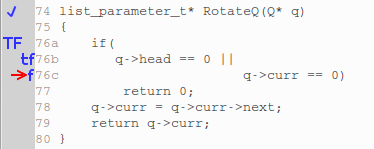
\includegraphics[width=0.8\columnwidth]{missed_decision_coverage.png}
    \caption{Decision Coverage Results show that {\tt RotateQ()} is never called
    with {\tt q->curr == 0} being true}
    \label{fig:decision_coverage_before}
\end{figure}

\begin{figure}
    \centering
    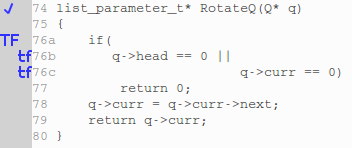
\includegraphics[width=0.8\columnwidth]{improved_decision_coverage.png}
    \caption{Decision Coverage Results show that {\tt RotateQ()} is never called
    with {\tt q->curr == 0} being true}
    \label{fig:improved_coverage}
\end{figure}


\section{Static Analysis}

\section{Conclusion}
Design of Experiments allows us to significantly reduce the test effort of our
face melting guitar application while still providing good test coverage.

\clearpage
\singlespace
\lstinputlisting[language=C++,label={lst:sort},caption={Selection Sort Implementation}]{sort.hpp}
\lstinputlisting[language=bash,label={lst:coverage_settings},caption={Setting up the BullseyeCoverage tool}]{bullseye_coverage_commands.sh}
\lstinputlisting[language=C++,label={lst:q_h},caption={Queue Implementation for
CSE531}]{q.h}
\lstinputlisting[language=C++,label={lst:q_test_cpp},caption={Initial Test code for CSE531}]{q.test.before.cpp}
\lstinputlisting[language=C++,label={lst:create_bad_condition},caption={New test
to improve condition coverage}]{create_bad_condition.cpp}

\doublespace

\printbibliography




\end{document}

